%https://docs.google.com/presentation/d/1NcWX0K9w16ijifVji554B3ElxtysNNXOaGcTpafr79o/edit?usp=sharing

%! TEX program = lualatex

\documentclass[nobackground,dvipsnames,table]{beamer}
\usepackage{tsc}
\usepackage{pdfpc}
\usepackage{pgfpages}
\usepackage{multimedia}

\mode<presentation>
{\usetheme{default}
	\usecolortheme{tsc}
	\setbeamercovered{transparent}
	\useinnertheme[shadow=false]{rounded}
	\usebackgroundtemplate{}
	\setbeamercolor*{frametitle}{parent=palette primary}
	\setbeamerfont{block title}{size={}}
	\setbeamertemplate{navigation symbols}{}
    \setbeamertemplate{itemize items}[circle]
     \setbeamertemplate{enumerate items}[circle]
}

%%%%%%%% edit hyperlink colors %%%%%%%%
\hypersetup{
  colorlinks   = true, 
  urlcolor     = tscurl, % color of external hyperlinks
  linkcolor    = white,   % color of internal links
}
%%% below command addresses log output error when trying to use \\ in \author %%%
\pdfstringdefDisableCommands{%
  \def\\{}%
}
%%%%% the below command allows custom highlights used in this presentation with \hlc %%%%%%
\makeatletter
\let\HL\hl
\renewcommand\hl{%
  \let\set@color\beamerorig@set@color
  \let\reset@color\beamerorig@reset@color
  \HL}
\makeatother

\newcommand{\hlc}[2][yellow]{{%
    \colorlet{foo}{#1}%
    \sethlcolor{foo}\hl{#2}}%
}

\title[Harassment and Hate Speech]{Harassment and Hate Speech}
%\subtitle{A document made with thought and care}

\author[]{Ina Kamenova, University of Massachusetts Lowell \\
Q. J. Yao, Lamar University \\ Mark Schneider}
%\institute[TSC]{\large Trust \& Safety Teaching Consortium}
\date[]{}
\subject{Trust and Safety}

\AddToShipoutPictureBG*{
  \AtPageLowerLeft{\hspace{-0.4cm}
    
\includegraphics[width=13.1cm]{img/consortium-image}}
}
% Change this to make a file with just slides, just notes or both
%\setbeameroption{hide notes}                 % Only slides
%\setbeameroption{show only notes}            % Only notes
\setbeameroption{show notes on second screen} % Both

\begin{document}

%\coverpage

%%%%%%%%%%%%%%%%%%%%%%%%%%%%%%%%%%%%%%%%%%%%%%%%%%%
%%%%%%%%%%%%%%%%%%%% SLIDE 1 %%%%%%%%%%%%%%%%%%%%%%
%%%%%%%%%%%%%%%%%%%%%%%%%%%%%%%%%%%%%%%%%%%%%%%%%%%
\begin{frame}
    \titlepage
\end{frame}

%%%%%%%%%%%%%%%%%%%%%%%%%%%%%%%%%%%%%%%%%%%%%%%%%%%
%%%%%%%%%%%%%%%%%%%% SLIDE 2 %%%%%%%%%%%%%%%%%%%%%%
%%%%%%%%%%%%%%%%%%%%%%%%%%%%%%%%%%%%%%%%%%%%%%%%%%%
\begin{frame}{Learning objectives}

\textbf{Today we will:}

\begin{itemize}
    \item Learn the definitions and types of online harassment and hate speech
    \item Learn the pervasive status quo of online harassment and hate speeches
    \item Learn how ethically and legally analyze online harassment and hate speech
    \item Learn how platforms and users handle online harassment and hate speech
\end{itemize}

\end{frame}


%%%%%%%%%%%%%%%%%%%%%%%%%%%%%%%%%%%%%%%%%%%%%%%%%%%
%%%%%%%%%%%%%%%%%%%% SLIDE 3 %%%%%%%%%%%%%%%%%%%%%%
%%%%%%%%%%%%%%%%%%%%%%%%%%%%%%%%%%%%%%%%%%%%%%%%%%%
\begin{frame}{A Definition of Online Harassment}

\begin{itemize}
    \item Definition: “interpersonal aggression or offensive behavior(s) that is communicated over the internet or through other electronic media.”(Slaughter \& Newsman 2022)
\end{itemize}

\end{frame}


%%%%%%%%%%%%%%%%%%%%%%%%%%%%%%%%%%%%%%%%%%%%%%%%%%%
%%%%%%%%%%%%%%%%%%%% SLIDE 4 %%%%%%%%%%%%%%%%%%%%%%
%%%%%%%%%%%%%%%%%%%%%%%%%%%%%%%%%%%%%%%%%%%%%%%%%%%
\begin{frame}{The Online Harassment Experience  Questionnaire 
\footnotesize{(OHEQ; for users to assess online harassment; Slaughter \& Newsman 2022)}}

\begin{itemize}
    \item Non-traumatic questions:  “I was impersonated by someone.”  “I was excluded from an online group.” “Offensive or hurtful comments were directed at me or posted about me or I was insulted.called names.” “Someone spread untrue rumors about me.”
    \item Potentially traumatic questions: “Someone threatened to harm me.” “I experienced unwanted sexual attention.” “My personal information was posted online where other could access it.” “Someone hacked, stole, or otherwise gained access to my online account(s) without my permission.” 
    \item Notes: those eight items are measured on a 6-point scale: 0 = never; 1 = less than once a month; 2 = 2 to 4 times a month; 3 = 2-4 times a week; 4 = daily; 5 = multiple times a day.
\end{itemize}

\end{frame}


%%%%%%%%%%%%%%%%%%%%%%%%%%%%%%%%%%%%%%%%%%%%%%%%%%%
%%%%%%%%%%%%%%%%%%%% SLIDE 5 %%%%%%%%%%%%%%%%%%%%%%
%%%%%%%%%%%%%%%%%%%%%%%%%%%%%%%%%%%%%%%%%%%%%%%%%%%
\begin{frame}{The State of Online Harassment 
(Pew Center 2021)}

\begin{itemize}
    \item Surveyed 10,093 American adults in September,  2020
    \item Roughly four-in-ten have experienced online harassment, half due to political reasons and half experiencing more severe behaviors
    \item Specifically, harassment includes:
    \begin{itemize}
        \item More severe forms: physical threats (14\%); stalking (11\%); sustained harassment (11\%); sexual harassment (11\%); all percentages raising from the past years
        \item Less severe forms: offensive name-calling (31\%); purposeful embarrassment (26\%); all percentages raising from the past years
    \end{itemize}
\end{itemize}

\scriptsize{Link to the course: \url{https://www.pewresearch.org/internet/2021/01/13/the-state-of-online-harassment/}}
\end{frame}



%%%%%%%%%%%%%%%%%%%%%%%%%%%%%%%%%%%%%%%%%%%%%%%%%%%
%%%%%%%%%%%%%%%%%%%% SLIDE 6 %%%%%%%%%%%%%%%%%%%%%%
%%%%%%%%%%%%%%%%%%%%%%%%%%%%%%%%%%%%%%%%%%%%%%%%%%%
\begin{frame}{The State of Online Harassment 
(Pew Center 2021, Cont.)}

\begin{itemize}
    \item Reasons for being a victim: Political reasons (50\%); gender (33\%); race/ethnicity (29\%); religion (19\%); sexual orientation (16\%); all percentages raising from the past years
    \item Venues of online harassment: Social media site (75\%); forum/discussion site (25\%); texting/messaging app (24\%); online gaming (16\%); personal email account (11\%); online dating site/app (10\%); multiple locations (41\%).
    \item 32\% believe social media addressing harassment poorly and 47\% think of it only fair. They proposed methods to reduce harassment: 1). Permanent suspension (51\%); real identity disclosure (48\%); criminal charges (43\%); proactive deletion (40\%); temporary suspension (32\%).
\end{itemize}
\end{frame}



%%%%%%%%%%%%%%%%%%%%%%%%%%%%%%%%%%%%%%%%%%%%%%%%%%%
%%%%%%%%%%%%%%%%%%%% SLIDE 7 %%%%%%%%%%%%%%%%%%%%%%
%%%%%%%%%%%%%%%%%%%%%%%%%%%%%%%%%%%%%%%%%%%%%%%%%%%
\begin{frame}{A Framework of Online-Harassment Assessment for Platform Regulation (Practices of Patio)}

\begin{itemize}
    \item When to moderate:
    \begin{enumerate}
        \item The following correspondence between the violator and the platform moderators is rough
        \item Platform users or the victim of the violation has no other way to address the violation   
    \end{enumerate}
\end{itemize}

\end{frame}


%%%%%%%%%%%%%%%%%%%%%%%%%%%%%%%%%%%%%%%%%%%%%%%%%%%
%%%%%%%%%%%%%%%%%%%% SLIDE 8 %%%%%%%%%%%%%%%%%%%%%%
%%%%%%%%%%%%%%%%%%%%%%%%%%%%%%%%%%%%%%%%%%%%%%%%%%%
\begin{frame}{A Framework of Online-Harassment Assessment for Platform Regulation (Practices of Patio, Cont.)}

\begin{itemize}
    \item Three criteria to decide if moderation (social sanction) is needed (Foley \& Gurakar, 2022):
    \begin{enumerate}
        \item Intensity: severity of the violation
        \item Specificity: the size of the target(s) of the violation; the more specific the more danger the violation is
        \item Persistence: frequency of the violation 
    \end{enumerate}
\end{itemize}
\end{frame}



%%%%%%%%%%%%%%%%%%%%%%%%%%%%%%%%%%%%%%%%%%%%%%%%%%%
%%%%%%%%%%%%%%%%%%%% SLIDE 9 %%%%%%%%%%%%%%%%%%%%%%
%%%%%%%%%%%%%%%%%%%%%%%%%%%%%%%%%%%%%%%%%%%%%%%%%%%
\begin{frame}{Online Hate Speech}

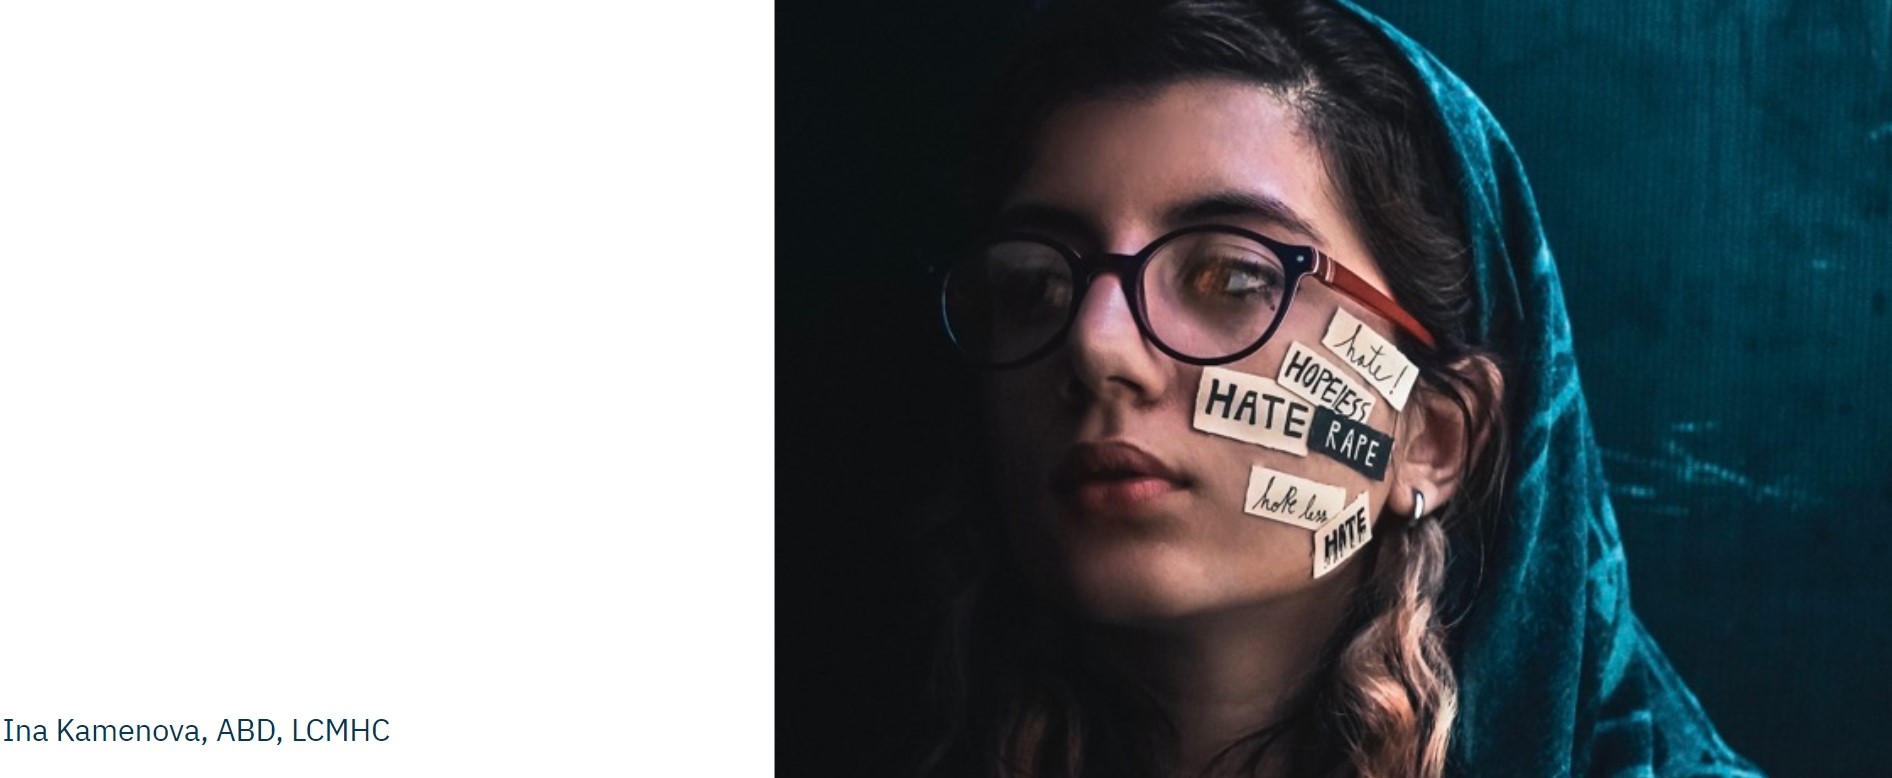
\includegraphics[scale=.28]{img/fig2.jpg}

\end{frame}



%%%%%%%%%%%%%%%%%%%%%%%%%%%%%%%%%%%%%%%%%%%%%%%%%%%
%%%%%%%%%%%%%%%%%%%% SLIDE 10 %%%%%%%%%%%%%%%%%%%%%%
%%%%%%%%%%%%%%%%%%%%%%%%%%%%%%%%%%%%%%%%%%%%%%%%%%%
\begin{frame}{What is hate speech?}

“a kind of speech act that contextually elicits certain detrimental social effects that are typically focused upon subordinated groups in a status hierarchy” \newline 

\scriptsize{(Demaske, 2021, p. 1014; United Nations, 2019, p. 2)}

\note[]{Definitions are variable and highly contested as legal concepts differ across EU and US and the landscape is shifting.  \newline \newline 
\scriptsize{Hietanen, M., \& Eddebo, J. (2022). Towards a Definition of Hate Speech—With a Focus on Online Contexts. Journal of communication Inquiry, 01968599221124309.}}

\end{frame}

\begin{frame}{Explicit v. implicit hate speech}

\begin{itemize}
    \item Explicit Hate Speech 
\begin{itemize}
    \item Directly identifies the target group (e.g., “Muslims”) and uses explicit attacks against the target group (e.g., slurs, explicit dehumanizing content). 
\end{itemize}
\item Implicit Hate Speech 
\begin{itemize}
    \item May not directly identify the target group (e.g., “terrorist sympathizers” instead of calling out “Muslims” in Islamaphobic content. 
\item Uses implicit language rather than explicit slur or attack (e.g., Hispanics live in sewage is an implicit form of dehumanization). 
\item Sometimes implicit hate speech is context specific (e.g., “cut down the tall trees” has a specific meaning in Rwanda).
\end{itemize}
\end{itemize}
\end{frame}




%%%%%%%%%%%%%%%%%%%%%%%%%%%%%%%%%%%%%%%%%%%%%%%%%%%
%%%%%%%%%%%%%%%%%% SLIDE 11 %%%%%%%%%%%%%%%%%%%%%%%
%%%%%%%%%%%%%%%%%%%%%%%%%%%%%%%%%%%%%%%%%%%%%%%%%%%
\begin{frame}{How is hate speech different from harassment?}

    \begin{itemize}
        \small{
        \item The message applies to a characteristic shared by a group of people 
        \item The impact is broader, described as concentric circles of hate impact. 
        \item The threat is potentially more unpredictable and unavoidable
        \item There can be intersections between harassment and hate speech, such as when targeted harassment includes hate speech, or when online hate speech also leads to harassment campaigns}
    \end{itemize}
    

\note[]{Castaño-Pulgarín, S. A., Suárez-Betancur, N., Vega, L. M. T. \& López, H. M. H. (2021). Internet, social media and online hate speech. Systematic review. \emph{Aggression and Violent Behavior, 58}(101608), 101608. \url{https://doi.org/10.1016/j.avb.2021.101608}}
\end{frame}

%%%%%%%%%%%%%%%%%%%%%%%%%%%%%%%%%%%%%%%%%%%%%%%%%%%
%%%%%%%%%%%%%%%%%%% SLIDE 12  %%%%%%%%%%%%%%%%%%%%%
%%%%%%%%%%%%%%%%%%%%%%%%%%%%%%%%%%%%%%%%%%%%%%%%%%%
\begin{frame}{Examples of hate speech categories}

\begin{itemize}
    \item Religious Hate Speech 
\end{itemize}
“inflammatory and sectarian language to promote hatred and violence against people on the basis of religious affiliation through the cyberspace” (Castaño-Pulgarín et al., 2021) 

\begin{itemize}
    \item Racist Speech 
\end{itemize}
As with all hate speech, racist messages can be direct (using slurs and describing characteristics associated with race unfavorably) or indirect: alluding to purity, nationality and oher coded concepts. 

\begin{itemize}
    \item Gender and Sexuality Hate Speech 
\end{itemize}
\end{frame}

%%%%%%%%%%%%%%%%%%%%%%%%%%%%%%%%%%%%%%%%%%%%%%%%%%%
%%%%%%%%%%%%%%%%%%%% SLIDE 13 %%%%%%%%%%%%%%%%%%%%%%
%%%%%%%%%%%%%%%%%%%%%%%%%%%%%%%%%%%%%%%%%%%%%%%%%%%
\begin{frame}{Comparative Legal Frameworks}

\textbf{US} \newline \newline  
In the US racist, sexist, and other hateful language online is not a crime. It can matter in criminal settings to categorize another crime as a hate crime and the offender may receive a hate crime enhancement to their sentence. \newline 

\textbf{UK \& Europe} \newline \newline 
The UK and Europe have much more stringent laws that make certain kinds of speech a crime in themselves. 

\end{frame}



%%%%%%%%%%%%%%%%%%%%%%%%%%%%%%%%%%%%%%%%%%%%%%%%%%%
%%%%%%%%%%%%%%%%%%%% SLIDE 14 %%%%%%%%%%%%%%%%%%%%%%
%%%%%%%%%%%%%%%%%%%%%%%%%%%%%%%%%%%%%%%%%%%%%%%%%%%
\begin{frame}{Freedom of Speech Exceptions in the US}

\begin{center}
    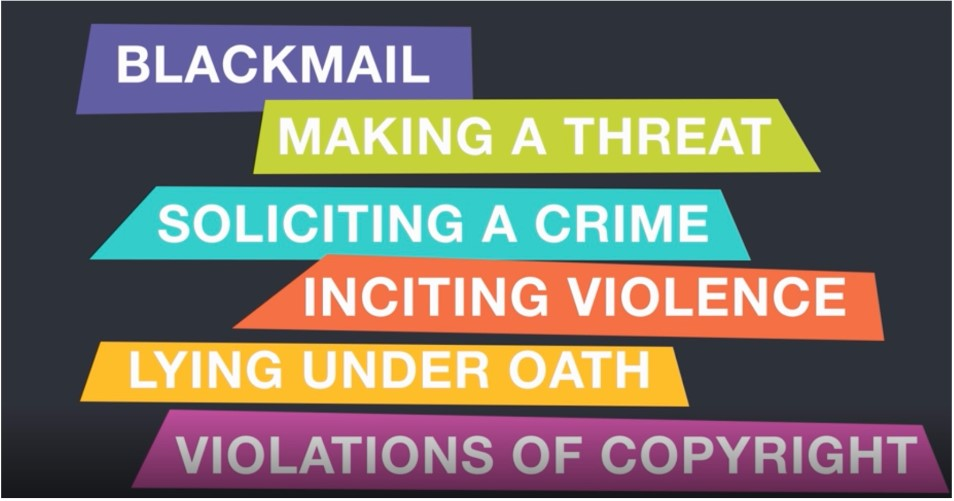
\includegraphics[width=\textwidth]{img/fig5.jpg} \newline   
\end{center}

The exceptions are very narrow and refer to criminal sanctions. Private institutions can regulate speech as they choose and have routinely done so.

\end{frame}


%%%%%%%%%%%%%%%%%%%%%%%%%%%%%%%%%%%%%%%%%%%%%%%%%%%
%%%%%%%%%%%%%%%%%%%% SLIDE 15 %%%%%%%%%%%%%%%%%%%%%%
%%%%%%%%%%%%%%%%%%%%%%%%%%%%%%%%%%%%%%%%%%%%%%%%%%%
\begin{frame}{Example cases of online hate speech and legal consequences }

Among many such cases, in July, 2022, a man was sentenced to 14 weeks imprisonment for a facebook post with racial slurs. 

\hlc[yellow]{Scott McCluskey, 43, posted a status update on his Facebook profile shortly after England lost to Italy on 11 July, Warrington magistrates court heard. He blamed “three ethnic players” for the defeat and then used a racial slur calling for them to be sacked.}

\hlc[yellow]{Describing it as a “foul offence which has far-reaching consequences”, district judge Nicholas Sanders sentenced McCluskey to 14 weeks’ imprisonment, suspended for 18 months, after the CPS successfully applied for the sentence to be strengthened because of the hate crime element.}

The UK has an “internet hate crime” reporting website. 

\note[]{
\url{https://www.report-it.org.uk/reporting_internet_hate_crime} \newline \newline 
\url{https://www.theguardian.com/world/2021/sep/08/man-sentenced-over-racist-post-after-euro-2020-final} \newline \newline 
\url{https://www.cps.gov.uk/mersey-cheshire/news/cheshire-man-sentenced-racist-abuse-england-players}
}
\end{frame}


%%%%%%%%%%%%%%%%%%%%%%%%%%%%%%%%%%%%%%%%%%%%%%%%%%%
%%%%%%%%%%%%%%%%%%%% SLIDE 16 %%%%%%%%%%%%%%%%%%%%%
%%%%%%%%%%%%%%%%%%%%%%%%%%%%%%%%%%%%%%%%%%%%%%%%%%%
\begin{frame}{Online Hate Speech Has Unique Features}
\begin{itemize}
    \footnotesize{
    \item Anonymity of the speaker. 
    \begin{itemize}
        \footnotesize{
        \item Even when the speaker is not anonymous, there is less risk to the speaker than when speaking directly in public, especially in the speaker’s community. }
    \end{itemize}

    \item Mobility and reach. 
    \begin{itemize}
        \footnotesize{
        \item Speech can be produced in one part of the world and copied and disseminated easily }
    \end{itemize}

    \item Durability. 
    \begin{itemize}
        \footnotesize{
        \item Sometimes speech can disappear and other times it can live forever, as it can be difficult to track down across platforms. 
        }
    \end{itemize}

    \item Size of audience. 
    \begin{itemize}
        \footnotesize{
        \item Online hate speech can reach a much wider or more niche audience much more easily than offline speech }
    \end{itemize}

    \item Ease of access. 
    \begin{itemize}
    \footnotesize{
        \item There is no need to join a group or physically opt to be in a space accepting of hate speech}
    \end{itemize}
    }
\end{itemize}


\note[]{Brown, A. (2018). What is so special about online (as compared to offline) hate speech? \emph{Ethnicities}, 18(3), 297–326. \url{https://doi.org/10.1177/1468796817709846}}
\end{frame}


%%%%%%%%%%%%%%%%%%%%%%%%%%%%%%%%%%%%%%%%%%%%%%%%%%%
%%%%%%%%%%%%%%%%%%%% SLIDE 17.1 %%%%%%%%%%%%%%%%%%%%%%
%%%%%%%%%%%%%%%%%%%%%%%%%%%%%%%%%%%%%%%%%%%%%%%%%%%
\begin{frame}{Impact of online hate speech}

\begin{itemize}
    \item Direct harm to targeted people and groups of people 

    \begin{itemize}
        \item E.g. psychological distress, defamation, social repercussions (e.g. in outing someone) 
    \end{itemize}

    \item Link with violent attacks
    \begin{itemize}
        \item E.g. linked with increasing hate crime and hateful ideology radicalization, which is thought to be related to increased single-actor attacks precipitated by participation in online, channels and other spaces elaborating on hateful ideologies or directly attacking people with targeted characteristics. 
    \end{itemize} 
\end{itemize}

\end{frame}

%%%%%%%%%%%%%%%%%%%%%%%%%%%%%%%%%%%%%%%%%%%%%%%%%%%
%%%%%%%%%%%%%%%%%%%% SLIDE 17.2 %%%%%%%%%%%%%%%%%%%%%%
%%%%%%%%%%%%%%%%%%%%%%%%%%%%%%%%%%%%%%%%%%%%%%%%%%%
\begin{frame}{Impact of online hate speech}

\begin{itemize}
    \item Influences Political Discourse 

    \begin{itemize}
        \item E.g. Hate speech online normalizes hateful ideologies, influences electoral process, in turn legislation and even judicial decisions. 
    \end{itemize}

    \item Disincentivizes others from participating in the discourse 
    \begin{itemize}
        \item E.g. people with targeted characteristics will be less likely to engage in public discourse knowing they will become targets for hate speech and harassment. Other people may also refrain because they do not want to read hateful content. 
    \end{itemize} 
\end{itemize}

\end{frame}


%%%%%%%%%%%%%%%%%%%%%%%%%%%%%%%%%%%%%%%%%%%%%%%%%%%
%%%%%%%%%%%%%%%%%% SLIDE 18.1 %%%%%%%%%%%%%%%%%%%%%
%%%%%%%%%%%%%%%%%%%%%%%%%%%%%%%%%%%%%%%%%%%%%%%%%%%
\begin{frame}{US Public Opinion Toward Hate Speech Leans Toward Moderating Hate Speech, Differs by Age}

\begin{center}
    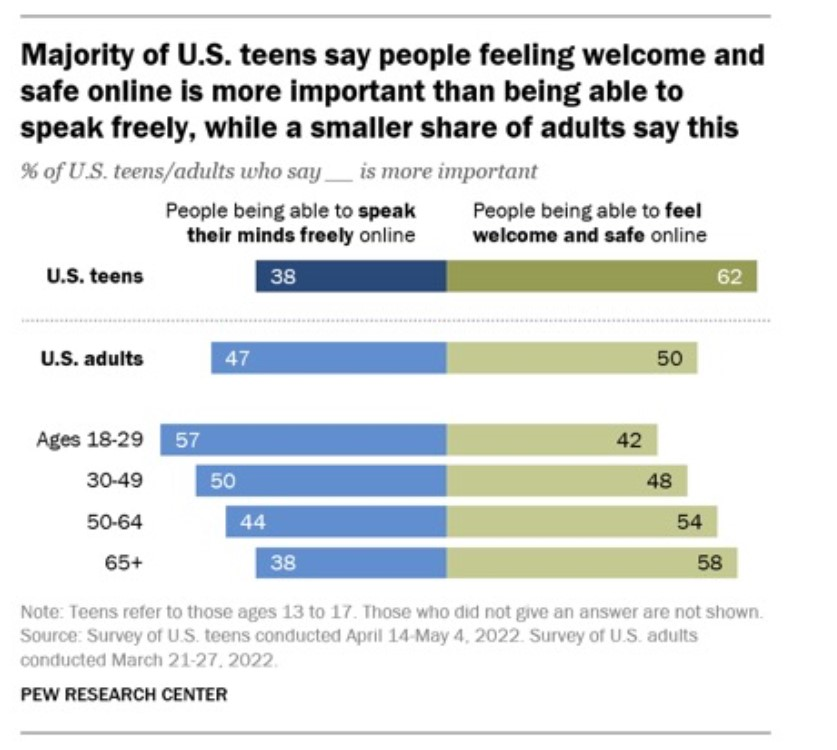
\includegraphics[scale=.5]{img/fig8.jpg}
\end{center}


\note[]{\url{https://www.pewresearch.org/fact-tank/2022/08/30/more-so-than-adults-u-s-teens-value-people-feeling-safe-online-over-being-able-to-speak-freely/}}
\end{frame}


%%%%%%%%%%%%%%%%%%%%%%%%%%%%%%%%%%%%%%%%%%%%%%%%%%%
%%%%%%%%%%%%%%%%%% SLIDE 18.2 %%%%%%%%%%%%%%%%%%%%%
%%%%%%%%%%%%%%%%%%%%%%%%%%%%%%%%%%%%%%%%%%%%%%%%%%%
\begin{frame}{US Public Opinion Toward Hate Speech Leans Toward Moderating Hate Speech, Differs by Age}

\begin{center}
    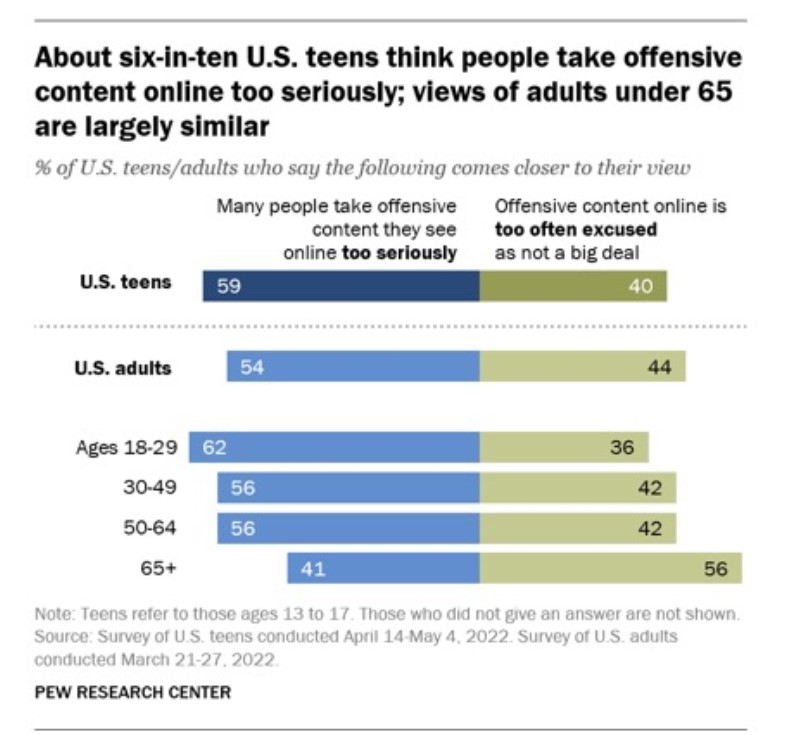
\includegraphics[scale=.5]{img/fig9.jpg}
\end{center}


\note[]{\url{https://www.pewresearch.org/fact-tank/2022/08/30/more-so-than-adults-u-s-teens-value-people-feeling-safe-online-over-being-able-to-speak-freely/}}
\end{frame}


%%%%%%%%%%%%%%%%%%%%%%%%%%%%%%%%%%%%%%%%%%%%%%%%%%%
%%%%%%%%%%%%%%%%%%%% SLIDE 19 %%%%%%%%%%%%%%%%%%%%%%
%%%%%%%%%%%%%%%%%%%%%%%%%%%%%%%%%%%%%%%%%%%%%%%%%%%
\begin{frame}{Public Opinion is Split Along Political Lines}
\hspace*{-6ex}
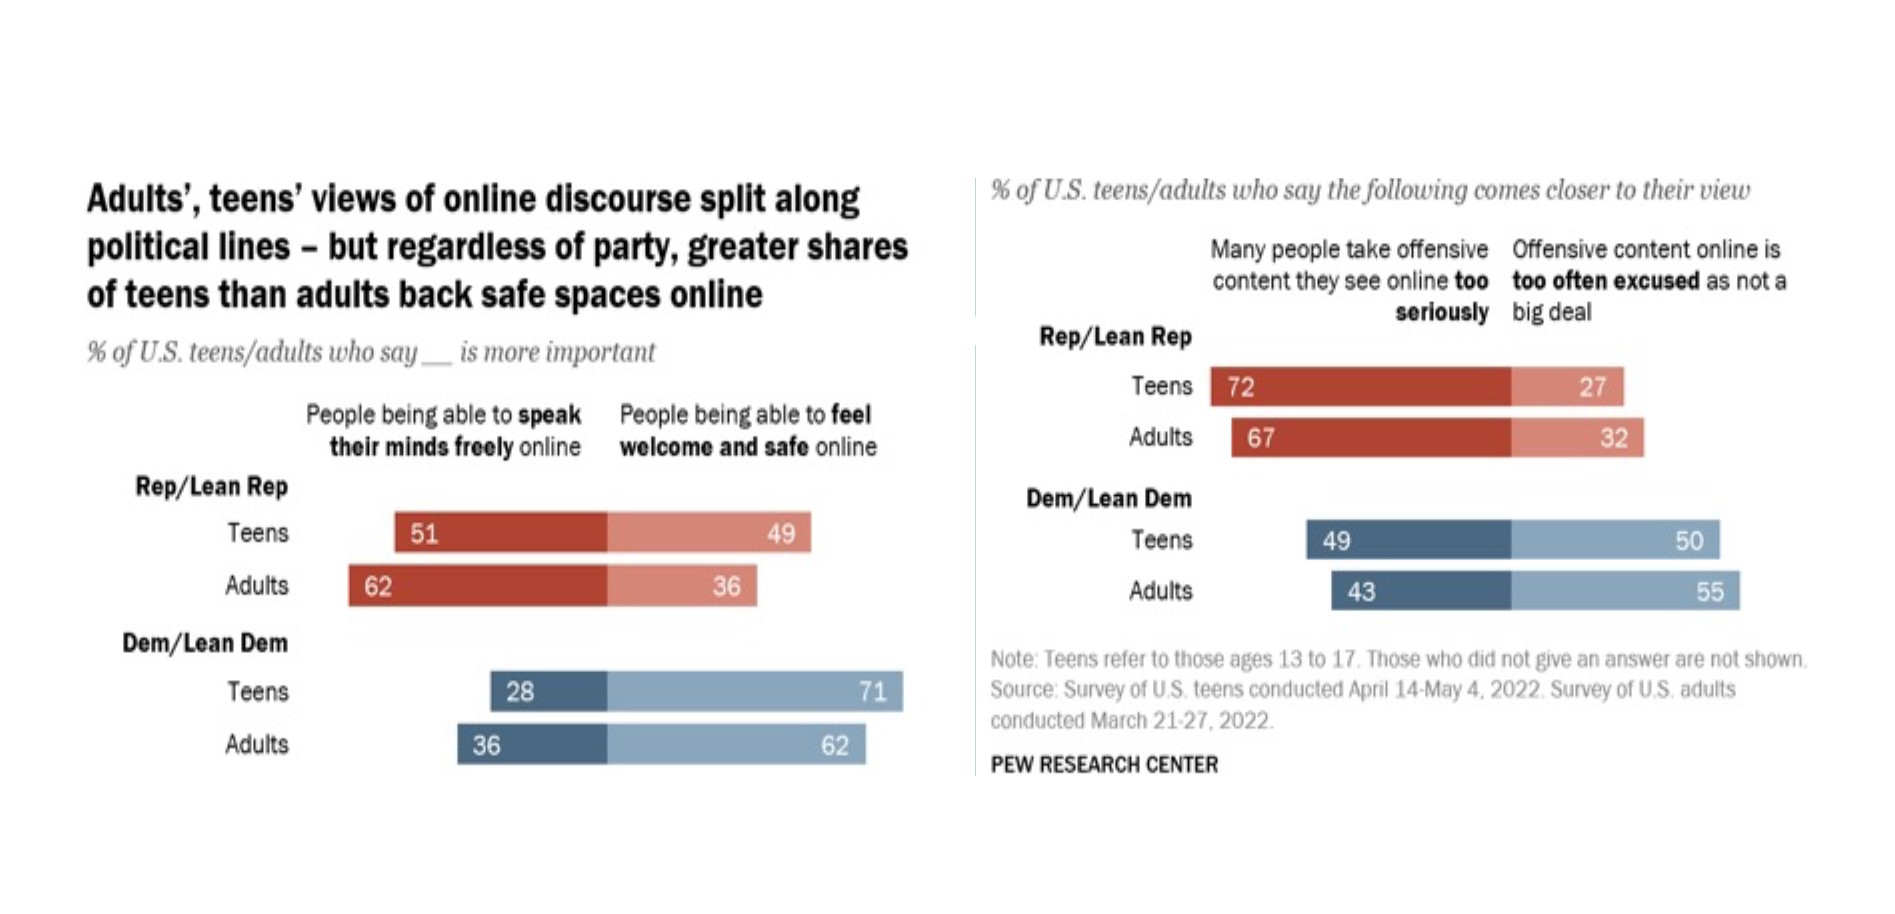
\includegraphics[scale=.33]{img/fig10.jpg}

\end{frame}



%%%%%%%%%%%%%%%%%%%%%%%%%%%%%%%%%%%%%%%%%%%%%%%%%%%
%%%%%%%%%%%%%%%%%%%% SLIDE 20 %%%%%%%%%%%%%%%%%%%%%%
%%%%%%%%%%%%%%%%%%%%%%%%%%%%%%%%%%%%%%%%%%%%%%%%%%%
\begin{frame}{Platform Response}

\begin{itemize}
    \item Hate speech, or hateful speech based on identity characteristics is mentioned in various ways in the content policy of platforms. 
    \item Check current platform policies for most up-to-date information. 
    \item These policies and practices are also changing as new legislation take effect in the EU and US. 
\end{itemize}

\end{frame}



%%%%%%%%%%%%%%%%%%%%%%%%%%%%%%%%%%%%%%%%%%%%%%%%%%%
%%%%%%%%%%%%%%%%%%%% SLIDE 21.1 %%%%%%%%%%%%%%%%%%%
%%%%%%%%%%%%%%%%%%%%%%%%%%%%%%%%%%%%%%%%%%%%%%%%%%%
\begin{frame}{Main Questions Investigated Differ by Discipline}

\textbf{Law}
\begin{itemize}
    \item In the United States, legal scholars primary ask questions about free speech and the limits of free speech. 
    \item Another currently contested area for legal scholars and legislators are regulatory expectations of platforms and to what extent offline speech principles apply such as the “public square” doctrine. 
\end{itemize}

\textbf{Psychology \& Sociology}
\begin{itemize}
    \item Considers social and individual impacts of hate speech. Research shows that there are similar effects to other traumatic events and effects vary by the type and amount of exposure. 
\end{itemize}

\note[]{\scriptsize{Often cited opinion pieces by legal scholars include: 
Balkin, Jack M., To Reform Social Media, Reform Informational Capitalism (September 6, 2021). Social Media, Freedom of Speech and the Future of Our Democracy; Lee Bollinger and Geoffrey R. Stone, eds., Forthcoming, Available at SSRN: \url{ https://ssrn.com/abstract=3925143} or \url{http://dx.doi.org/10.2139/ssrn.3925143} \newline \newline 

\url{https://www.americanbar.org/groups/crsj/publications/human_rights_magazine_home/the-ongoing-challenge-to-define-free-speech/in-the-age-of-socia-media-first-amendment/} \newline 
\url{https://scholarlycommons.law.case.edu/cgi/viewcontent.cgi?referer=&httpsredir=1&article=1076&context=jolti}}}
\end{frame}

%%%%%%%%%%%%%%%%%%%%%%%%%%%%%%%%%%%%%%%%%%%%%%%%%%%
%%%%%%%%%%%%%%%%%% SLIDE 21.2 %%%%%%%%%%%%%%%%%%%%%
%%%%%%%%%%%%%%%%%%%%%%%%%%%%%%%%%%%%%%%%%%%%%%%%%%%
\begin{frame}{Main Questions Investigated Differ by Discipline}

\textbf{Criminology \& Security Studies}
\begin{itemize}
    \item Hate speech can be produced by hate groups as well as by individuals and has been linked with online adicaization and hate crimes and terrorist acts. 
\end{itemize}

\textbf{Political Science}
\begin{itemize}
    \item Primarily focused on hate speech as political speech and the effects on political discourse, elections \& legislation. 
\end{itemize}

\textbf{CS \& IS}
\begin{itemize}
    \item Primarily asks questions about automatic detection and moderation of hate speech. 
\end{itemize}

\note[]{\scriptsize{Often cited opinion pieces by legal scholars include: 
Balkin, Jack M., To Reform Social Media, Reform Informational Capitalism (September 6, 2021). Social Media, Freedom of Speech and the Future of Our Democracy; Lee Bollinger and Geoffrey R. Stone, eds., Forthcoming, Available at SSRN: \url{ https://ssrn.com/abstract=3925143} or \url{http://dx.doi.org/10.2139/ssrn.3925143} \newline \newline 

\url{https://www.americanbar.org/groups/crsj/publications/human_rights_magazine_home/the-ongoing-challenge-to-define-free-speech/in-the-age-of-socia-media-first-amendment/} \newline 
\url{https://scholarlycommons.law.case.edu/cgi/viewcontent.cgi?referer=&httpsredir=1&article=1076&context=jolti}}}
\end{frame}


%%%%%%%%%%%%%%%%%%%%%%%%%%%%%%%%%%%%%%%%%%%%%%%%%%%
%%%%%%%%%%%%%%%%%%%% SLIDE 22 %%%%%%%%%%%%%%%%%%%%%%
%%%%%%%%%%%%%%%%%%%%%%%%%%%%%%%%%%%%%%%%%%%%%%%%%%%
\begin{frame}{In-class Discussion \newline \emph{\small{Freedom of Speech and Hate Speech.}}}

Where do you stand on issues of hate speech and freedom of speech? \newline 

Are there settings that customarily already place restrictions to free speech? \newline 

How effective are current automated detection methods in your opinion? \newline 

\note[]{Customize and flesh out these answers as needed and pair students or assign small groups with specific readings and handouts based on the readings.}

\end{frame}



%%%%%%%%%%%%%%%%%%%%%%%%%%%%%%%%%%%%%%%%%%%%%%%%%%%
%%%%%%%%%%%%%%%%%%%% SLIDE 23 %%%%%%%%%%%%%%%%%%%%%%
%%%%%%%%%%%%%%%%%%%%%%%%%%%%%%%%%%%%%%%%%%%%%%%%%%%
\begin{frame}{In-class \& At-Home Team Exercise \newline \emph{\small{Compare current platform policies.}}}

What, if any mention is there of hate speech? 
How has it changed over time? (Use archived previous versions.) 
How do you think hate speech policies vary based on:

\begin{itemize}
    \footnotesize{
    \item The type of product or service (e.g., social media network, digital marketplace, search engine);
    \item The types of abuse, misuse, and disruptive conduct the company must address;
    \item The set of values that the company upholds;
    \item The demographics of its customer base;
    \item The countries in which it operates;
    \item The size of and maturity level of the company.
    }
\end{itemize}

\note[]{Links to the current policies of several platforms: 
\url{https://www.tiktok.com/community-guidelines?lang=en\#39}}
\end{frame}



%%%%%%%%%%%%%%%%%%%%%%%%%%%%%%%%%%%%%%%%%%%%%%%%%%%
%%%%%%%%%%%%%%%%%%%% SLIDE 24 %%%%%%%%%%%%%%%%%%%%%%
%%%%%%%%%%%%%%%%%%%%%%%%%%%%%%%%%%%%%%%%%%%%%%%%%%%
\begin{frame}{Sources of Information}
Since this a rapidly developing field, the most recent information on new scholarship and information can be very field-specific. Below is a list of sources that are have specifically dedicated to Online Trust \& Safety Issues, including free speech. 

\begin{itemize}
    \item Journal of Online Trust and Safety 
    \item Arbiters of Truth Series of the Lawfare Podcast 
\end{itemize}

\end{frame}

%%%%%%%%%%%%%%%%%%%%%%%%%%%%%%%%%%%%%%%%%%%%%%%%%%%
%%%%%%%%%%%%%%%%%%%% SLIDE 25 %%%%%%%%%%%%%%%%%%%%%%
%%%%%%%%%%%%%%%%%%%%%%%%%%%%%%%%%%%%%%%%%%%%%%%%%%%
\begin{frame}{Areas for Further Study \& Recent Issues}
Further Study 
\begin{itemize}
    \item Repeated calls for interdisciplinary collaboration to make progress on these issue. 
    \item The magnitude of the issue is difficult to pin down and scholars are calling for more research. 
    \item Multi-platform cooperation and academic-industry collaborations. 
    \item Moral and legal principles are continuously under debate alongside technological capabilities to execute desired policies for intervention and prevention 
\end{itemize}

Recent issues 
\begin{itemize}
    \item Legislation debates 
    \item Tech industry layoffs of teams responsible for hate speech detection and moderation 
\end{itemize}

\end{frame}

%\backpage

\end{document}